\documentclass{article}
\usepackage{graphicx}

\setlength{\parskip}{\medskipamount}
\makeatletter
\let \@sverbatim \@verbatim
\def \@verbatim {\@sverbatim \verbatimplus}
{\catcode`'=13 \gdef \verbatimplus{\catcode`'=13 \chardef '=13 }}
\makeatother

\title{Introduction to IT Security\\
\medskip
\large Homework 7 -- SQL Injections}
\author{Abraham Murciano}

\begin{document}

\maketitle

\section{RedTiger's Hackit}

\subsection{Level 1}

The challenge for the first level is to obtain the password for the user Hornoxe. The webpage, whose interface is visible in figure \ref{1.1.ui}, consists of two fields to enter a username and password, and some descriptive text on some category labelled `1'.

\begin{figure}[htbp]\
	\centering
	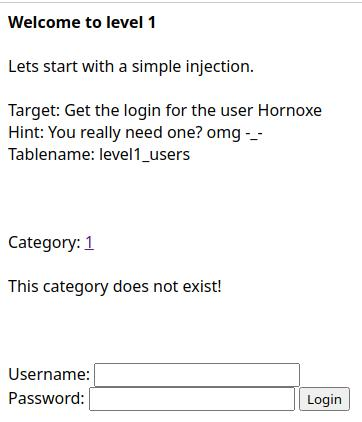
\includegraphics[scale=0.6]{1.1.ui.jpg}
	\caption{UI of website for level 1}
	\label{1.1.ui}
\end{figure}

The first thing I tried was to enter some text into the username and password fields to see if my input was displayed anywhere in the site, or included in the page source. This path did not yield any success.

The next attempt was to input the text \verb`Hornoxe' and sleep(20)` into the username field, and see if there was a twenty second delay in the processing of the submission. Unfortunately there wasn't, which meant that the username field was likely invulnerable to SQL injections. Trying something similar with the password field was equally unsuccessful.

The next thing to try was the category. After performing some inspection, I found that clicking on the link on the number 1 passed a url parameter to the page of the form ``\verb`?cat=1`''. When the page loads with that parameter, instead of saying ``This category does not exist'', it displayed some text about that category. This behaviour would lead us to believe that there is some SQL statement which retrieves the description of category 1 which looks something like this.

\begin{verbatim}
	SELECT [some columns] FROM categories WHERE id=1
\end{verbatim}

In order to confirm this suspicion, and to find our if this input was vulnerable to SQL injections, I requested the site with ``\verb`?cat=1 and sleep(20)--`'' as the URL parameter. Luckily, the page took twenty seconds to load, so it seems that our suspicions are correct.

What I wanted to do next was to cause the where condition to fail, and then union whatever data I wanted (the password of user Hornoxe) to the query result, so the site would display that instead of the description of the category. However, in order to union something to the result, I needed to know how many columns were being selected, since the second query that I was going to union to the existing one needed to use the same number of columns.

So I tried to select one column, then two, then three, and when I tried with four I was able to see what I had selected on the page. The URL parameters looked like this.

\begin{verbatim}
	?cat=0 union select 1,2,3,4--
\end{verbatim}

After running this, I was able to see the numbers three and four displayed on the site, so we can infer that the third and fourth columns of the query result are what is displayed on the site.

Changing the query to the following one successfully displayed the password ``\verb`thatwaseasy`'' on the page.

\begin{verbatim}
	?cat=0 union select 1,2,username,password from level1_users--
\end{verbatim}

\subsection{Level 2}

Here we are displayed with a simple login with a username and password field. Trying various malicious inputs in the username field was unsuccessful, which led me to believe that the username field is not vulnerable to SQL injections. That left only the password field.

A typical SQL query to authenticate a user looks something like the following.

\begin{verbatim}
	SELECT * FROM users WHERE username='[username]' and
	password='[password]'
\end{verbatim}

Assuming this was what the query in question looked like, I attempted to enter ``\verb`' or 1=1--`'' as the password. However, that resulted in the page showing a PHP error which meant the query had failed.

I suspected that perhaps there was an important part of SQL code after the location which the password was being inserted, and since I had two dashes in the password, I was commenting that important code out. I therefore needed to modify my password so that I would not comment any code out, while still being a syntactically correct query.

The password ``\verb`' or 1=1 or '`'' accomplished just that and successfully logged me in.

\section{Zixem}

\subsection{Level 1}

We are tasked with obtaining the version of the database engine and username of the database user. The page we are targeting has no input fields, but it does have a URL parameter \verb`?id=1`. Replacing the URL parameter with \verb`?id=1 and 1=2` causes some of the data on the page to disappear, which indicates that the query returned an empty result set.

Next, I tried to find out how many columns there were in the select statement that was being run. To do this I used the following URL parameters, each time adding more numbers to the end until I didn't receive and error. With this I learned that there have to be three columns selected in the union.

\begin{verbatim}
	?id=1 and 1=2 union select 1,2,3--
\end{verbatim}

This time, I was able to see the numbers one and two in the page content, so I replaced them with \verb`user()` and \verb`version()` like so.

\begin{verbatim}
	?id=1 and 1=2 union select user(),version(),3--
\end{verbatim}

This revealed that the version is 5.6.33-log and the user is zixem@localhost.

\subsection{Level 2}

In this challenge we are facing a website with a URL parameter of the form \verb`?showprofile=4`. The site then shows the user ID, username, and age of the selected profile.

The first thing I tried was to replace the four with a single quote. That caused the site to display a MySQL syntax error message which occurred ``near ` ` ' ' ' at line 1''. Since there were five single quotes in the error message, the first and last ones are part of the error message, used to quote actual SQL code. That leaves three quotes which were in the SQL query. This indicates that whatever input I give is put in single quotes, probably because the profile id field is of type string.

Next, I want the query to always fail, so that I can union my own data to the result set. The following URL parameter achieves that. The final single quote must be there to match the quote that was intended to go after the four.

\begin{verbatim}
	?showprofile=4' and 0=1 and '
\end{verbatim}

The next step is to determine how many columns are being selected. I requested the site with a few similar URL parameters, until one did not give me an error.

\begin{verbatim}
	?showprofile=4' and 0=1 union select 'one','two','three','four
\end{verbatim}

This showed `one'. `two', and `three' on the page, but did not show `four'. So finally I ran the following query to reveal the user and version.

\begin{verbatim}
	?showprofile=4' and 0=1 union select user(),version(),'','
\end{verbatim}

\subsection{Level 3}

This challenge is practically identical in structure to the previous one. Attempting to run a slightly altered version of the final URL parameter from the previous level gave the following error message.

\begin{verbatim}
	...syntax to use near 'uni select user(),version(),'',''' at...
\end{verbatim}

As the error message shows, the word `union' is being converted to `uni'. To combat this, I attempted to use the word `unionon', and that worked. The final query is shown below.

\begin{verbatim}
	?item=3' and 0=1 union select user(),version(),'','
\end{verbatim}

\subsection{Level 4}

Again, this challenge was identical to the second one, other than there being a different number of columns. The first thing I tried was to use the same query as the one from Level 2, then when I was told there was a different number of columns, I added some more until I got the right answer. This is the final query.

\begin{verbatim}
	?ebookid=7' and 0=1 union select user(),version(),'','','
\end{verbatim}

\end{document}
